\documentclass{article}

% Packages
\usepackage{graphicx}
\usepackage{listings}
\usepackage{xcolor}
\usepackage{indentfirst}
\usepackage{hyperref}
\usepackage{hyperref} \hypersetup{
  colorlinks=true,
  linkcolor=black,
  citecolor=black,
  urlcolor=blue,
}

% Set highlighting for source code
\definecolor{codegreen}{rgb}{0,0.6,0}
\definecolor{codegray}{rgb}{0.5,0.5,0.5}
\definecolor{codepurple}{rgb}{0.58,0,0.82}
\definecolor{bg}{rgb}{0.97,0.97,0.97}
\lstdefinestyle{code} {
  backgroundcolor=\color{bg},
  commentstyle=\color{codegreen},
  keywordstyle=\color{magenta},
  stringstyle=\color{codepurple},
  basicstyle=\ttfamily\footnotesize,
  breakatwhitespace=false,
  breaklines=true,
  captionpos=b,
  keepspaces=true,
  showspaces=false,
  showstringspaces=false,
  showtabs=false,
  tabsize=2
}
\lstset{style=code}

\title{%
  CSCI 4511W Final Project \\
  \large Quantum machine learning in bioinformatics
}
\author{Brian Cooper \\ coope824@umn.edu \\ University of Minnesota}
\date{\today}

\begin{document}
\maketitle

\section*{Abstract}
  Quantum computing is an emergent field that provides promising potential for bioinformatics, the interdisciplinary field combining computational methods and problems in biology, such as DNA alignment and sequencing. Among various problems, classification is a common task in bioinformatics machine learning tasks for identifying and predicting classes of objects, such as organisms or genes. Using a quantum variant of the classical support vector machine, a quantum model can be created in a similar manner to a classical support vector machine model for making predictions. Applied quantum computing is quite new, and it is not commonly used in modern bioinformatics experiments. Here, it is demonstrated that quantum computing frameworks, although in their infancy, can be used to design and test classification models, and are robust enough to prototype. The accuracy of the quantum support vector machine is demonstrated to compare competitively with its classical counterpart, despite claims that quantum computing is not yet mature enough for widespread use. These results demonstrate that quantum computing may be ready for testing in modern experiments extending beyond bioinformatics into other scientific domains.

\section*{Problem Overview}
  Bioinformatics is, in deep simplification, the combination of computational thinking with problems in bioinformatics. Such problems range from analyzing genetic expression from proteomic (protein) data and other data (such as sequenced DNA and RNA), constructing phylogenetic trees to determine structure among organisms, and developing medicine to counteract disease. Machine learning is a tool that is often used in bioinformatics problems, due to the usefulness of being able to accurately predict properties of data such as its structure and applied functions. This fascinates me, so I decided to analyze bioinformatics classification problems, with the twist of comparing quantum variants of such tasks to their classical counterparts. Specifically, I wanted to compare quantum algorithms (algorithms designed to run on a quantum computer) to classical algorithms (algorithms designed to run on a ``classical,'' or traditional, computer). Classical computers run on binary logic, meaning the information stored on them is stored in discrete bits that take on a state of either 0 or 1. Quantum computers, on the other hand, operate on quantum information, which is stored in \textit{quantum bits} or ``qubits.'' As qubits are subject to quantum phenomena, they can take on any number of states between and including 0 and 1 with a concept known as ``superposition.'' This can explored further in Martin Giles' explanation of quantum computers on MIT Technology Review~\cite{giles}, along with some more details about the mystical nature of quantum computers. Quantum computing is relatively novel and undeveloped, despite a rich theoretical history and decades of thought, dating back to Richard Feynman's idea of a ``computer that models nature'' (and possibly before, unrecorded). Classical computers have been used extensively to solve machine learning problems, but quantum computing is a relatively new and smaller space. Through this project, I hoped to answer a basic question: are quantum computing algorithms useful and practical for working with bioinformatics machine learning problems? At the very least, I wanted to create a foundation for implementing the algorithms detailed below, one that can be expanded upon in the future. \\

  The problem outlined here compares the performance of quantum machine learning support vector machine algorithms to their classical counterparts on bioinformatics classification problems.

\section*{Related Work}
  Quantum computing, machine learning, and bioinformatics are established, yet highly plastic fields. Some researchers from the somewhat disparate disciplines have combined their efforts. Quantum machine learning, a synthesis of quantum computing and machine learning, is built upon the foundations of quantum mechanics and artificial intelligence. Such research efforts customarily uses classical machine learning approaches as a baseline for analyzing corresponding quantum counterparts, however they differ in their proposals for analysis and applied solutions. Biamonte, et al.~\cite{biamonte} argue that machine learning has a bright future when utilizing quantum processing power, and they mention that significant advancements have been made when it comes to hardware. They clarify that certain devices (such as annealing quantum computers) \textit{have} been built with apparently large qubit counts (2000, for example), although they do not communicate with each other well at such a scale yet, so there is ample room for improvement. Dunjko, et al.~\cite{dunjko} primarily discussed complexity improvements for quantum methods. Finally, the paper by Schuld, et al.~\cite{schuld} solely zones in on classification and clustering methods (although in great depth) and emphasizes that we need to be careful in the wishful optimism of quantum computing's usefulness to machine learning -- especially considering its infancy. Despite this caution, the paper expresses hope and considers the field to have a promising future. \\

  When it comes to practicality, it is argued in~\cite{biamonte} that the foundation for quantum machine learning algorithms is strong, yet considerably limited by hardware and software challenges. An important point in~\cite{schuld} is that the ability to simulate the actual, concrete learning process in quantum systems is unsatisfactorily documented, and thus requires more development. \\

  Two dominant machine learning tasks, classification and clustering, are commonly used in modern problems. Although my problem is focused on classification, it is useful to recognize clustering methods within the domain to discover auxiliary information. Each is composed of varying depths of analysis in associated algorithms (such as support vector machines with different kernels for classification and k-means for clustering). Biamonte, et al.~\cite{biamonte} provide several runtime complexity difference estimates for various quantum algorithms. Quantum support vector machines, for example, are estimated to perform faster with an $O(\log{N})$ speedup (exponential speedup), albeit with certain constraints~\cite{aaronson}. In \cite{dunjko}, a quadratic improvement is common, and even exponential in relatively short time scales (converges to quadratic as $t \rightarrow \infty$). Schuld, et al.~\cite{schuld} describe the ``toolbox of quantum algorithms'' to actually be quite well-established and offer promising speedups. The authors detail in great depth various concrete examples of learning problems which are performed on classical computers and consider the same task on a quantum computer. An example they provide is from~\cite{lloyd} which proposes that a quantum version of the nearest-centroid algorithm~\cite{centroid} is more efficient than the polynomial runtime required for the same task on a classical computer, even despite the auxiliary quantum operations that need to be performed. \\

  Bioinformatics, in contrast to the analysis of quantum machine learning above, is built upon the foundations of biology, machine learning, and statistical methods. Similar tasks, namely classification and clustering, have been used since the advent of the study of bioinformatics. In~\cite{ward}, the structures of mRNA, tRNA, and rRNA are predicted by testing the energy levels required to form a structure. A structure can be predicted with a certain accuracy by measuring such energy levels. Confidence is proportional to a lower energy level, since it takes less energy to form that structure. It is unlikely for a structure requiring a high energy level to form since it is biologically inefficient, and this data is used to train a machine learning classification model using support vector machines. Other classification problems are introduced and suggested in~\cite{byvatov}, where support vector machines are demonstrated to perform well on tasks such as identifying molecules that modulate the function of certain protein receptors, compared to other approaches such as neural networks. \\

  Changing perspective, clustering methods are also used in bioinformatics. Higham, et al.~\cite{higham} cover in great depth the mechanics of spectral clustering, and offer light into its use in bioinformatics. In particular, they address gene expression activity across various tissue samples, and explain how clustering is a natural approach for resolving such gene activity. In~\cite{olman}, the overwhelming amount of modern data (``big data'') is addressed and clustering approaches are suggested for reducing the complexity of bioinformatics problems. A minimum spanning tree representation is utilized within a clustering approach within a software called CLUMP are introduced, and drastic time complexity improvement is promised with using such software. \\

  Combining bioinformatics with quantum machine learning is relatively new and unexplored space, at least in the public domain. Despite this, I think it is clear that there is much potential in the future of computing.

\section*{Approach}
  Quantum computing is very much in its infancy, but there have been strides from major companies such as IBM and Microsoft to open the field to interested individuals. There are several quantum computing projects being worked on right now with public access, including (but certainly not limited to):

  \begin{itemize}
    \ind
    \item IBM Q~\cite{ibm} (further described below)
    \item Microsoft Quantum~\cite{msft}
    \item Rigetti Quantum Cloud Services~\cite{rigetti}
    \item D-Wave Ocean~\cite{dwave}
  \end{itemize}

  Qiskit~\cite{qiskit}, a Python quantum computing SDK and framework from IBM designed to simulate quantum processes, was used to design the models and execute the classification tests. Qiskit provides two distinct methods for performing quantum computing experiments:

    \begin{itemize}
      \item{Running tasks on real quantum computing hardware (connected to IBM Q computers with an API)}
      \item{A built-in quantum hardware simulator for performing experiments on a classical computer}
    \end{itemize}

  The simulator was chosen, as I do not have any academic credit required to perform experiments on real quantum computing hardware. This necessarily rules out any accurate analysis of the time and space complexities, since quantum computing mathematics is calculated within a classical computer environment. Quantum computing algorithms are, of course, designed to be run on quantum hardware, so the computational time and space cannot be accurately gauged in this manner. Qiskit does provide GPU acceleration support through its QCGPU communication package~\cite{qcgpu}. Further, Qiskit makes use of a ``quantum assembly'' language called \textit{OpenQASM}, which allows implementing quantum circuitry close to the hardware. \\

  Multivariate data was selected from the UCI Machine Learning Repository~\cite{uci}. Instances from five datasets were used:

    \begin{itemize}
      \item Breast Cancer Wisconsin (Diagnostic)~\cite{bc}
      \item Ecoli~\cite{ecoli}
      \item Yeast~\cite{yeast}
      \item Parkinson's~\cite{park}
      \item Statlog Heart~\cite{heart}
    \end{itemize}

  All of the above datasets have been previously used for classification training and testing with various methods, including (but certainly not limited to) various kernel SVM methods.

\section*{Experiment Design and Results}
  \begin{center}
    \textit{Note: all of the code, with comments and explanations, can be seen in the appendix. The input dataset files are not included in the appendix, nor is the Jupyter notebook that utilizes the source code to execute the tests and render the result graphics.}
  \end{center}

  Qiskit comes packaged with a convenient API, allowing lots of room for parameter tuning and custom design. This allows various things to be set and tweaked, including the kernel (and direct manipulation of it using the kernel trick), quantum parameters such as shots (described in the following paragraph), and the feature map (which maps feature vectors -- vectors based on input data -- into a space with a more useful dimensionality for computation; highly dependent on the nature and distribution of the input data). Since there is so much flexibility, I fixed some of these parameters to focus the experiments as more of an A/B test between classical and quantum models, rather than primarily trying to improve the learned classes and result metrics. \\

  A specific parameter that can be specified when constructing an algorithm in Qiskit is the number of \textit{shots}, which specifies how many times a quantum circuit is repeated. The reason it's desirable to repeat the circuit multiple times is to gradually build up distribution statistics of the logical circuit results. In Qiskit, this number is 1024 by default. I reduced this value to 256 to speed up the computation time. \\

  A support vector machine with a radial basis kernel was chosen (same kernel for both types of support vector machines -- classical and quantum). The radial basis kernel is defined by a \textit{radial basis function}, or \textit{RBF}, and the kernel function is displayed in Figure \ref{fig:kernel}. In the RBF kernel, \textbf{x} and \textbf{x}$^\prime$ represent feature vectors (as samples) in the input data, and $\sigma$ is a free variable, set to 1 in these experiments. It is important to mention that a core difference of the quantum support vector machine, despite having the same kernel as the classical support vector machine, uses a quantum processor to directly estimate the kernel in the feature space.

  \begin{figure}[h]
    \[ K(\textbf{x,~x}^\prime) = \exp(- \frac{||\textbf{x - x}^\prime||}{2 \sigma^2}) \]
    \caption{\label{fig:kernel}Radial basis function kernel.}
  \end{figure}

  Each of the datasets was split into 70\% testing data and 30\% training data. Principal component analysis (PCA) dimensionality reduction was used to reduce the space to two dimensions, which matches the number of qubits used in the quantum support vector machine. The data spaces, after dimensionality reduction, can be visualized in Figure \ref{fig:data}. \\

  \begin{figure}[h]
    \centering
    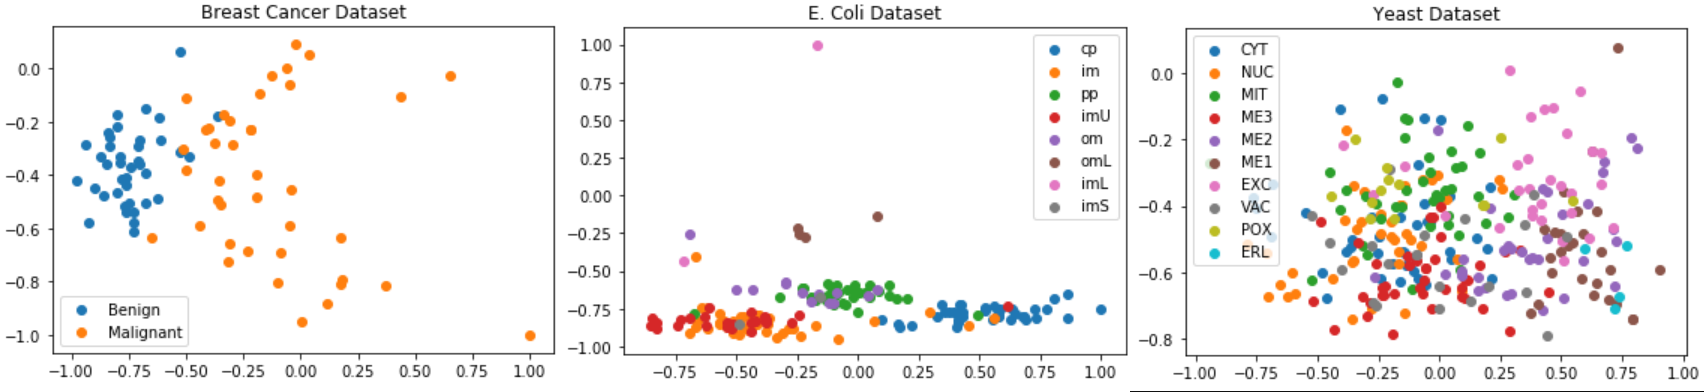
\includegraphics[width=1\textwidth]{img/vis1.png}
    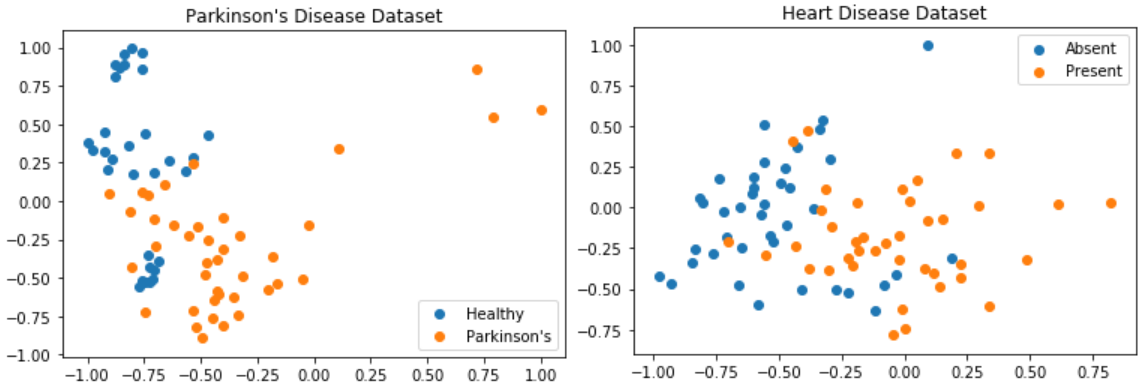
\includegraphics[width=0.7\textwidth]{img/vis2.png}
    \caption{\label{fig:data}Visualization of the data.}
  \end{figure}

  Table \ref{table:accuracy} shows the accuracy results of the classical and quantum support vector machine experiments on all three datasets. Figure \ref{fig:results} shows the same results visually. \\

  \begin{table}[h]
    \centering
    \begin{tabular}{c|c|c|}
    \cline{2-3}
                                  & Classical SVM & Quantum SVM \\ \hline
    \multicolumn{1}{|c|}{Breast Cancer} & 75\%          & 90\%        \\ \hline
    \multicolumn{1}{|c|}{E. Coli}   & 90\%          & 60\%        \\ \hline
    \multicolumn{1}{|c|}{Yeast}   & 45\%          & 43\%        \\ \hline
    \multicolumn{1}{|c|}{Parkinson's}   & 40\%          & 60\%        \\ \hline
    \multicolumn{1}{|c|}{Statlog Heart}   & 60\%          & 55\%        \\ \hline
    \end{tabular}
    \caption{\label{table:accuracy}Model accuracy results.}
  \end{table}

  \hfill \break

  \begin{figure}[h]
    \centering
    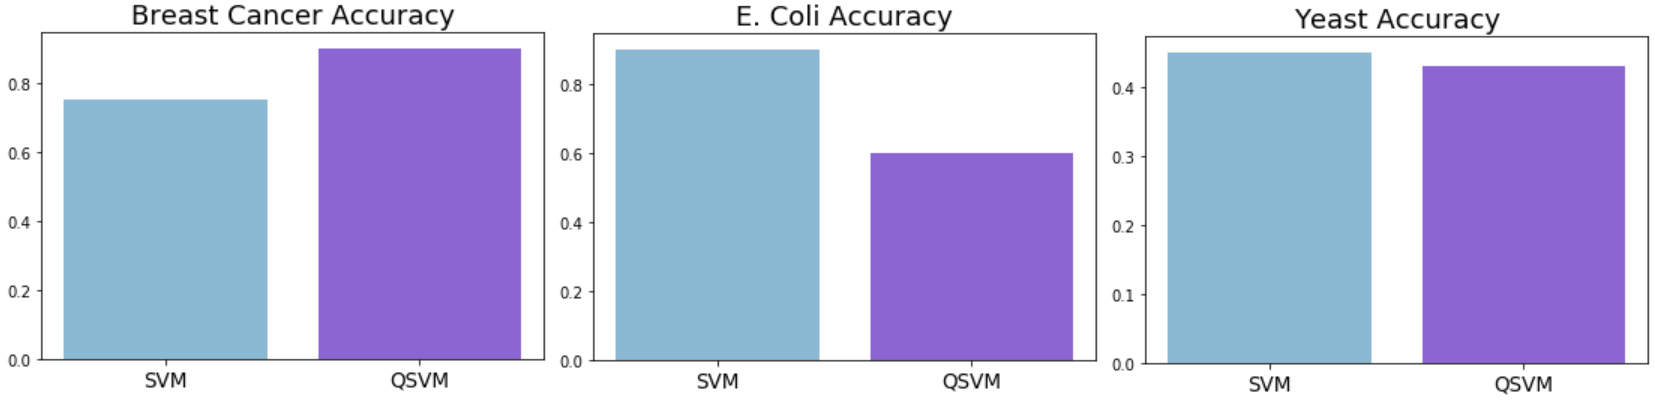
\includegraphics[width=1\textwidth]{img/acc1.png}
    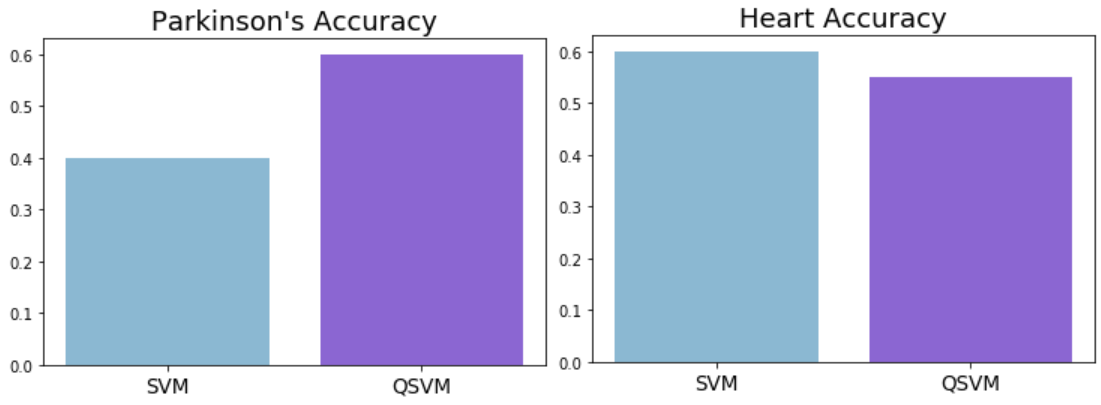
\includegraphics[width=0.7\textwidth]{img/acc2.png}
    \caption{\label{fig:results}Visual model accuracy results.}
  \end{figure}

\section*{Analysis}
  Even when reducing the number of shots to 256, the quantum algorithm tests still took a very long time compared to the classical algorithm tests with the same RBF kernel. Overall, each of the five quantum algorithm runs (with all 256 shots included) took several hours, while all five of the classical algorithms completed in under a minute. It is important to recall that these quantum experiments were performed on a simulator rather than physical quantum devices (such as those of IBM Q), and the performance would likely improve on a physical quantum computer. To adjust this, the backend for each Qiskit Aqua (Qiskit's artificial intelligence suite) parameter list can be changed in the file ``svm.py'' in the provided source code. Assuming the QASM simulator is accurate and factors in noise and other environmental factors, using a physical IBM Q backend should produce similar results to those above with faster speed. There is some commented code in ``svm.py'' that allows usage of GPU acceleration for the circuit backend. Augmenting the circuit runs with a GPU would likely improve the performance as well. \\

  The experiments only compare QSVM and SVM with an RBF kernel. More SVM kernels can be used on the data, and more algorithms aside from SVM can be used on the data. This would provide more insight in the experiments. As mentioned previously, the intention is not to improve the models, but rather to demonstrate that quantum implementations are indeed effective and usable. \\

  The quantum implementation of SVM created a model with better accuracy on the breast cancer dataset (90\% vs. 75\%) and the Parkinson's dataset (60\% vs. 40\%). For the yeast and heart datasets, the quantum algorithm was very close behind in accuracy (43\% vs. 45\% and 55\% vs. 60\%, respectively). The E. coli dataset is the only dataset where the RBF SVM had a very large accuracy improvement over the quantum SVM (60\% vs. 90\%). As mentioned in the previous paragraph, it would be ideal to perform other quantum machine learning algorithms on the data to provide more benchmarks. Precision, recall, and F1-score are some measures that can further be used to analyze the experimental output. \\

  As Qiskit is a young project, many of the algorithms contained within are largely proof-of-concept. As the project matures, the algorithms will be optimized and will naturally become more performant. The documentation will concurrently be improved, especially considering that Qiskit is an open-source project. Other quantum computing projects will follow suit: over time, utilizing quantum technology will become more accessible and robust. This is an exciting and rapidly-changing field that may be very useful in all sorts of applications. Even though the experiments only involved comparing the two SVM algorithms currently shipped with Qiskit, this demonstration shows that it is possible to already use quantum algorithms without too much difficulty. Qiskit in particular abstracts away from the physics and digital logic quite highly, at least for quickly spinning up an algorithm without too much tuning. Machine learning models built with a quantum foundation may be a useful tool to add when trying different algorithms on data.

\section*{Conclusion}
  This work challenges the notion that quantum computing algorithms are not practical for modern use. The hardware is indeed limited, however, Qiskit and other frameworks enable convenient quantum algorithm usage and lower the barrier for entry by opening the source code to the public. As machine learning uses become more prominent and ubiquitous, quantum computing frameworks may facilitate and augment the field with complexity reduction and new approaches. \\

  Overall, the quantum computing space is exciting and certainly could be something to consider for future scientific work as the technology advances. Quantum computers are slated to be excellent at solving optimization problems, which are at the core of artificial intelligence and machine learning problems. Thus, it is likely that bioinformatics will enjoy a surge of innovation as quantum computers establish their place in society, and, necessarily, other disciplines as a whole.

\newpage
\bibliographystyle{plain}
\raggedright
\bibliography{./final-project}

\section*{Appendix}

\subsection*{data.py}
  \begin{center}
    \textit{This file processes the input data and prepares it for experimentation.}
  \end{center}

  \begin{lstlisting}[language=Python]
  import matplotlib.pyplot as plt
  import numpy as np
  import pandas as pd
  import scipy
  from mpl_toolkits.mplot3d import Axes3D
  from scipy.linalg import expm
  from sklearn import datasets
  from sklearn.decomposition import PCA
  from sklearn.model_selection import train_test_split
  from sklearn.preprocessing import StandardScaler, MinMaxScaler

  # ============================================================= #
  # Data preparation - PCA dimensionality reduction, etc.         #
  # ============================================================= #
  def prepare_data(data, target, n, training_size, test_size, class_labels):
    # Split data for training and testing
    sample_train, sample_test, label_train, label_test = \
        train_test_split(data, target, test_size=0.3, random_state=12)

    # Standarize for Gaussian around 0 with unit variance
    std_scale = StandardScaler().fit(sample_train)
    sample_train = std_scale.transform(sample_train)
    sample_test = std_scale.transform(sample_test)

    # Reduce number of features to number of qubits
    pca = PCA(n_components=n).fit(sample_train)
    sample_train = pca.transform(sample_train)
    sample_test = pca.transform(sample_test)

    # Scale to range (-1, +1) for convenience
    samples = np.append(sample_train, sample_test, axis=0)
    minmax_scale = MinMaxScaler((-1, 1)).fit(samples)
    sample_train = minmax_scale.transform(sample_train)
    sample_test = minmax_scale.transform(sample_test)

    # Pick training size samples from each distribution
    training_input = {key: (sample_train[label_train == k, :])[:training_size] \
        for k, key in enumerate(class_labels)}
    test_input = {key: (sample_train[label_train == k, :])[training_size:(
        training_size+test_size)] for k, key in enumerate(class_labels)}

    return sample_train, label_train, training_input, test_input

  # ============================================================= #
  # Breast cancer dataset                                         #
  # ============================================================= #
  def breast_cancer(training_size, test_size, n, PLOT_DATA):
    class_labels = [r'Benign', r'Malignant']

    df = pd.read_csv('datasets/breast-cancer-wisconsin.csv', header=None)
    df = df.replace({'B':0, 'M':1})
    data = df.iloc[:,2:]
    target = df.iloc[:,1]

    sample_train, label_train, training_input, test_input = \
        prepare_data(data, target, n, training_size, test_size, class_labels)

    if PLOT_DATA:
        for k in range(2):
            label = 'Benign' if k is 0 else 'Malignant'

            plt.scatter(sample_train[label_train == k, 0][:training_size],
                        sample_train[label_train == k, 1][:training_size],
                        label=label)

        plt.title("Breast Cancer Dataset")
        plt.legend()
        plt.show()

    return sample_train, training_input, test_input, class_labels

  # ============================================================= #
  # Ecoli dataset                                                 #
  # ============================================================= #
  def ecoli(training_size, test_size, n, PLOT_DATA):
    class_labels = [r'cp', r'im', r'pp', r'imU', r'om', r'omL', r'imL', r'imS']

    df = pd.read_csv('datasets/ecoli.csv', header=None)
    df = df.replace({'cp':0, 'im':1, 'pp':2, 'imU':3, 'om':4, 'omL':5, \
        'imL':6, 'imS':7})
    data = df.iloc[:,1:8]
    target = df.iloc[:,8]

    sample_train, label_train, training_input, test_input = \
        prepare_data(data, target, n, training_size, test_size, class_labels)

    if PLOT_DATA:
        for k in range(8):
            if k == 0:
                label = 'cp'
            elif k == 1:
                label = 'im'
            elif k == 2:
                label = 'pp'
            elif k == 3:
                label = 'imU'
            elif k == 4:
                label = 'om'
            elif k == 5:
                label = 'omL'
            elif k == 6:
                label = 'imL'
            else:
                label = 'imS'

            plt.scatter(sample_train[label_train == k, 0][:training_size],
                        sample_train[label_train == k, 1][:training_size],
                        label=label)

        plt.title("E. Coli Dataset")
        plt.legend()
        plt.show()

    return sample_train, training_input, test_input, class_labels

  # ============================================================= #
  # Yeast dataset                                                 #
  # ============================================================= #
  def yeast(training_size, test_size, n, PLOT_DATA):
    class_labels = [r'CYT', r'NUC', r'MIT', r'ME3', r'ME2', r'ME1', r'EXC', \
        r'VAC', r'POX', r'ERL']

    df = pd.read_csv('datasets/yeast.csv', header=None)
    df = df.replace({'CYT':0, 'NUC':1, 'MIT':2, 'ME3':3, 'ME2':4, 'ME1':5, \
        'EXC':6, 'VAC':7, 'POX':8, 'ERL':9})
    data = df.iloc[:,1:9]
    target = df.iloc[:,9]

    sample_train, label_train, training_input, test_input = \
        prepare_data(data, target, n, training_size, test_size, class_labels)

    if PLOT_DATA:
        for k in range(10):
            if k == 0:
                label = 'CYT'
            elif k == 1:
                label = 'NUC'
            elif k == 2:
                label = 'MIT'
            elif k == 3:
                label = 'ME3'
            elif k == 4:
                label = 'ME2'
            elif k == 5:
                label = 'ME1'
            elif k == 6:
                label = 'EXC'
            elif k == 7:
                label = 'VAC'
            elif k == 8:
                label = 'POX'
            else:
                label = 'ERL'

            plt.scatter(sample_train[label_train == k, 0][:training_size],
                        sample_train[label_train == k, 1][:training_size],
                        label=label)

        plt.title("Yeast Dataset")
        plt.legend()
        plt.show()

    return sample_train, training_input, test_input, class_labels

  # ============================================================= #
  # Parkinson's dataset                                           #
  # ============================================================= #
  def parkinson(training_size, test_size, n, PLOT_DATA):
    class_labels = [r'Healthy', r'Parkinson\'s']

    df = pd.read_csv('datasets/parkinsons.csv', header=None)
    data = df.iloc[:,1:23]
    target = df.iloc[:,23]

    sample_train, label_train, training_input, test_input = \
        prepare_data(data, target, n, training_size, test_size, class_labels)

    if PLOT_DATA:
        for k in range(2):
            label = 'Healthy' if k is 0 else 'Parkinson\'s'

            plt.scatter(sample_train[label_train == k, 0][:training_size],
                        sample_train[label_train == k, 1][:training_size],
                        label=label)

        plt.title("Parkinson's Disease Dataset")
        plt.legend()
        plt.show()

    return sample_train, training_input, test_input, class_labels

  # ============================================================= #
  # Heart dataset                                                 #
  # ============================================================= #
  def heart(training_size, test_size, n, PLOT_DATA):
    class_labels = [r'Absent', r'Present']

    df = pd.read_csv('datasets/heart.csv', header=None)
    df = df.replace({1:0, 2:1})
    data = df.iloc[:,0:13].astype(float)
    target = df.iloc[:,13].astype(float)

    sample_train, label_train, training_input, test_input = \
        prepare_data(data, target, n, training_size, test_size, class_labels)

    if PLOT_DATA:
        for k in range(2):
            label = 'Absent' if k is 0 else 'Present'

            plt.scatter(sample_train[label_train == k, 0][:training_size],
                        sample_train[label_train == k, 1][:training_size],
                        label=label)

        plt.title("Heart Disease Dataset")
        plt.legend()
        plt.show()

    return sample_train, training_input, test_input, class_labels
  \end{lstlisting}

\subsection*{svm.py}
  \begin{center}
    \textit{This file sets up the quantum and classical support vector machines.}
  \end{center}

  \begin{lstlisting}[language=Python]
  from datasets import *
  import numpy as np
  from qiskit.aqua.utils import split_dataset_to_data_and_labels
  from qiskit.aqua.input import ClassificationInput
  from qiskit.aqua import run_algorithm
  # from qiskit_qcgpu_provider import QCGPUProvider

  # ============================================================= #
  # Quantum support vector machine                                #
  #   train_input:  training set                                  #
  #   test_input:   testing set                                   #
  #   n:            projected input dimensionality                #
  # ============================================================= #
  def quantum_svm(train_input, test_input, class_labels, n):
    temp = [test_input[k] for k in test_input]
    total_array = np.concatenate(temp)

    # Select parameters based on number of classes in data
    if len(class_labels) > 2:
        aqua_dict = {
            'problem': {'name': 'classification', 'random_seed': 100},
            'algorithm': {
                'name': 'QSVM'
            },
            'feature_map': {'name': 'SecondOrderExpansion', 'depth': 2, \
                'entangler_map': [[0, 1]]},
            'multiclass_extension': {'name': 'AllPairs'},
            'backend': {'name': 'qasm_simulator', 'shots': 256}
        }
    else:
        aqua_dict = {
            'problem': {'name': 'classification', 'random_seed': 100},
            'algorithm': {
                'name': 'QSVM'
            },
            'feature_map': {'name': 'SecondOrderExpansion', 'depth': 2, \
                'entangler_map': [[0, 1]]},
            'backend': {'name': 'qasm_simulator', 'shots': 256}
        }

    # Use the QCGPUProvider for improved performance
    # If using, make sure to enable the import code on line 6
    # backend = QCGPUProvider().get_backend('qasm_simulator')

    algo_input = ClassificationInput
    algo_input.training_dataset = train_input
    algo_input.test_dataset = test_input
    algo_input.datapoints = total_array

    # Run the quantum SVM algorithm
    # Use the second version if using the QCGPUProvider backend (GPU)
    result = run_algorithm(aqua_dict, algo_input)
    # result = run_algorithm(aqua_dict, algo_input, backend=backend)

    # Print model values
    # for k,v in result.items():
    #   print("'{}' : {}".format(k, v))

    return result

  # ============================================================= #
  # Classical support vector machine (Radial basis kernel)        #
  #   train_input:  training set                                  #
  #   test_input:   testing set                                   #
  #   n:            projected input dimensionality                #
  # ============================================================= #
  def classical_svm(train_input, test_input, class_labels, n):
    temp = [test_input[k] for k in test_input]
    total_array = np.concatenate(temp)

    # Select parameters based on number of classes in data
    if len(class_labels) > 2:
        aqua_dict = {
            'problem': {'name': 'classification', 'random_seed': 100},
            'algorithm': {
                'name': 'SVM'
            },
            'multiclass_extension': {'name': 'AllPairs'}
        }
    else:
        aqua_dict = {
            'problem': {'name': 'classification', 'random_seed': 100},
            'algorithm': {
                'name': 'SVM'
            }
        }

    algo_input = ClassificationInput
    algo_input.training_dataset = train_input
    algo_input.test_dataset = test_input
    algo_input.datapoints = total_array

    # Run the classical SVM algorithm
    result = run_algorithm(aqua_dict, algo_input)

    # Print model values
    #  for k,v in result.items():
    #      print("'{}' : {}".format(k, v))

    return result
  \end{lstlisting}

\end{document}
